\section{Empirical Application}\label{sec:empirical}

\subsection{Data and Empirical Design}\label{subsec:empirical_data_design}

\paragraph{Data.}

We estimate the model using daily returns for a large cross-section of NYSE stocks and a high-dimensional set of predictors capturing variation in the information environment. The stock sample consists of firms that are continuously listed on the New York Stock Exchange between 2010 and 2017. Returns are measured at the daily frequency.

Our main predictors are the 180 daily news-topic attention series of \citet{Bybee2021}, constructed from the full text of the \textit{Wall Street Journal} using an unsupervised Latent Dirichlet Allocation (LDA) model. The LDA model assigns each article a vector of topic shares, which \citet{Bybee2021} aggregate to the daily level to measure attention to a broad set of business, economic, political, and social topics. Table~\ref{tab:news_topics} reports the full set of topics.
To complement these news-based measures, we add 10 aggregate macro-financial time series that are widely monitored by market participants, including Treasury yields, the VIX, oil prices, and other indicators of aggregate financial and macroeconomic conditions. The final predictor vector therefore combines 180 news-topic attention series with 10 macro-financial variables.
This predictor set is intentionally broad. News topics capture heterogeneous dimensions of public information, while the macro-financial variables summarize aggregate market conditions that may affect expected returns across many firms. There is little ex ante theoretical guidance about which of these signals, if any, should forecast the return of a given stock at a given point in time. The setting is therefore well suited for our empirical exercise: agents face a high-dimensional forecasting problem and must select a sparse subset of potentially relevant signals.

We use innovations rather than levels. Topic attention and macro-financial variables are persistent, and their levels largely capture slow-moving variation in news coverage and aggregate conditions. To isolate unexpected changes in the information environment, we estimate an AR($p$) process separately for each predictor series, choosing the lag length $p$ by the Akaike Information Criterion (AIC). We define $X_t$ as the vector of residuals from these regressions. Thus, $X_t$ contains innovations in both news-topic attention and macro-financial conditions.
Consistent with the model, returns are measured as log returns,
$r_{i,t} = \log(R_{i,t})$,
where $R_{i,t}$ is the gross return of stock $i$ on day $t$.
The final sample contains 1{,}620 stocks, 190 predictor series, and 1{,}889 trading days. The predictor set consists of 180 news-topic attention series and 10 macro-financial time series. Table~\ref{tab:summary_stats} reports summary statistics for returns, topic levels, and topic innovations.


\begin{table}[H]
\centering
\caption{Summary Statistics}
\label{tab:summary_stats}

\begin{tabular}{lccccccc}
\toprule
Variable & Mean & SD & Min & Max & Skewness & Kurtosis & $N$ \\
\midrule
Log return
    & 0.000 & 0.021 & $-$1.964 & 2.051 & $-$0.587 & 101.917 & 3,060,180 \\
\addlinespace
Topic level
    & 0.006 & 0.004 & 0.000 & 0.116 & 3.662 & 33.361 & 340,020 \\
Topic innovation
    & 0.000 & 0.003 & $-$0.054 & 0.062 & 1.885 & 16.019 & 339,840 \\
\bottomrule
\end{tabular}

\medskip
\begin{minipage}{0.95\textwidth}
\footnotesize
\textit{Note:} The table reports summary statistics for daily stock returns and news-topic attention measures. Returns are daily log returns, $r_{i,t}=\log(R_{i,t})$, for NYSE-listed stocks from 2010 to 2017. Topic attention series are constructed from the Wall Street Journal following \citet{Bybee2021}. Topic innovations are residuals from topic-specific AR($p$) models, where the lag length is selected by the Akaike Information Criterion.
\end{minipage}
\end{table}


\subsection{Implementing the Learning Rule}\label{subsec:empirical_learning_rule}

\paragraph{Estimation Strategy.}

The empirical strategy mirrors the two central objects of the model. Agents form beliefs about return predictability using a misspecified perceived law of motion (PLM), and these beliefs affect prices through the actual law of motion (ALM). Because investors' beliefs are not observed, we first reconstruct the belief process implied by the learning rule and then examine whether the resulting belief path helps explain realized returns through the ALM.\footnote{The empirical implementation differs from the theoretical setup in three respects. First, agents estimate the PLM using a rolling window of fixed length rather than geometrically declining weights. This specification is commonly used in empirical forecasting applications with potentially time-varying relations and closely follows \citet{Chinco2019}. Second, agents estimate a full LASSO regression rather than the soft-thresholding approximation used in the theory. The two coincide under orthonormal regressors, and the approximation remains accurate when regressors are weakly correlated. Consistent with this assumption, Figure~\ref{fig:corr_heatmap} in Appendix~\ref{app:tab_figures} shows that topic-attention innovations are close to contemporaneously uncorrelated, while Table~\ref{tab:cross_lag_correlations} documents only small cross-lag correlations. Third, we allow lagged topic innovations to enter the PLM, allowing investors to learn from delayed effects of news topics on returns.}

Let $x_t \in \mathbb{R}^k$ denote the vector of topic-attention innovations observed on
day $t$. For a rolling window of length $s$, define
\begin{equation}
X_t
=
\begin{bmatrix}
x_{t-s}^\top \\
x_{t-s+1}^\top \\
\vdots \\
x_{t-1}^\top
\end{bmatrix},
\qquad
r_{i,t}
=
\begin{bmatrix}
r_{i,t-s+1} \\
r_{i,t-s+2} \\
\vdots \\
r_{i,t}
\end{bmatrix}.
\end{equation}
Each row of $X_t$ contains the topic innovations available at a given date, while each
column tracks one topic over the estimation window. For each stock $i$ and each window
ending at $t-1$, the investor estimates a LASSO coefficient vector
\begin{equation}
\hat{\beta}_{i,t}
=
\arg\min_{\beta \in \mathbb{R}^k}
\left\{
\frac{1}{s}
\sum_{\tau=t-s}^{t-1}
\left(r_{i,\tau+1}-x_\tau^\top \beta\right)^2
+
\lambda \sum_{j=1}^{k} |\beta_j|
\right\}.
\end{equation}
The empirical PLM is therefore
\begin{equation}\label{eq:empirical_plm}
r_{i,\tau+1}
=
x_\tau^\top \beta_{i,t}
+
\eta_{i,\tau+1},
\qquad
\tau=t-s,\ldots,t-1.
\end{equation}
The coefficient vector $\hat{\beta}_{i,t}$ is indexed by both stock and time. Its
$j$-th element measures the perceived predictive content of topic $j$ for stock $i$ at
date $t$. Repeating this estimation window by window yields a stock-specific belief path
$\hat{\beta}_{i,t}$. The corresponding belief index,
\[
    f_{i,t} = x_t^\top \hat{\beta}_{i,t},
\]
is the one-step-ahead return forecast implied by the investor's PLM.

We use the estimated belief path to estimate the actual law of motion implied by the
asset-pricing equation. For each stock $i$, we estimate
\begin{equation}\label{eq:empirical_alm}
r_{i,t+1}
=
c_i
+
\log\!\left(1-\kappa_i e^{x_t^\top \hat{\beta}_{i,t}}\right)
-
\log\!\left(1-\kappa_i e^{x_{t+1}^\top \hat{\beta}_{i,t+1}}\right)
+
\varepsilon_{i,t+1},
\end{equation}
where $c_i$ captures average return components outside the model. The parameter
$\kappa_i$ measures the strength of the feedback from perceived predictability to realized
returns and is estimated by nonlinear least squares. Identification is based on time-series
variation in the belief index $f_{i,t}=x_t^\top\hat{\beta}_{i,t}$. If the first-stage LASSO never
selects any predictor, $f_{i,t}$ is constant and $\kappa_i$ is not identified. Conversely, if the
penalty is too weak, the belief index is dominated by estimation noise. The empirical
implementation therefore requires sparse but non-degenerate first-stage selection.

Prior to implementing our estimation strategy, we fix the rolling window length and calibrate only the LASSO penalty ($\lambda$).
Throughout the empirical analysis, we use one lag of the predictor innovations.
We set the baseline window to $s=252$ trading days, corresponding to one calendar year of daily data.\footnote{The choice of 252 trading days is motivated by the natural information horizon of a calendar year: corporate earnings cycles, annual reports, and macroeconomic policy reviews all operate at this frequency, making it a reasonable upper bound on how long a piece of news remains statistically relevant for forecasting returns.}
In our setting, window length is a proxy for memory length: how far back information remains relevant for forecasting next-day returns.
This choice also aligns with standard annual governance and model review cycles in practice.

Because the penalty is not known ex ante, we select $\lambda$ via a cross-sectional hold-out procedure, reserving 20\% of stocks as a tuning set while the remaining 80\% form the estimation sample.
The standard approach in the literature is to cross-validate on a predictive loss such as MSE or out-of-sample $R^2$ \citep{Chinco2019, Gu2020, Feng2020}.
For our purposes, however, the object of interest is not predictive accuracy per se but the identification of $\kappa$ which would confirm the validity of our CMCE model.
So the correct penalty should produce sparse, non-degenerate beliefs that yield a statistically significant second-stage estimate.
We show in Appendix~\ref{app:oracle} that a composite objective that combines the first-stage in-sample fit with the second-stage significance of $\kappa$ performs well in recovering the true penalty in a simulated environment.
The optimization based on this objective yields $\lambda = 3.224 \times 10^{-3}$, which is then fixed and applied across all estimation stocks.

\subsection{Baseline Estimation Results}\label{subsec:empirical_baseline_results}

\paragraph{Estimation Results.}

Having calibrated the learning parameters, we now implement the model on the remaining 80\% of stocks that were not used during calibration. For each stock, we estimate the PLM in equation~(\ref{eq:empirical_plm}) using a rolling-window LASSO with the previously selected parameter values. This procedure delivers a time series of belief coefficients ${\hat{\beta}_{i,t}}$ and corresponding one-step-ahead forecasts, which we summarize in Table~\ref{tab:summary_stats_lasso}.

\begin{table}[H]
\centering
\caption{First-Stage LASSO Estimation Results}
\label{tab:summary_stats_lasso}

\begin{tabularx}{\textwidth}{@{}>{{\small}}Xccccccc@{}}
\toprule
 & mean & std & median & min & max & p05 & p95 \\
\midrule
In-sample $R^2$   & 0.0249 & 0.0416 & 0.0071 & $-$0.0073 & 0.2790 & $-$0.0040 & 0.1124 \\
Out-of-sample $R^2$ & $-$0.0115 & 0.0234 & $-$0.0035 & $-$0.3677 & 0.0054 & $-$0.0488 & $-$0.0001 \\
Selection rate    & 0.0222 & 0.0350 & 0.0071 & 0.0000 & 0.2464 & 0.0000 & 0.0971 \\
\bottomrule
\end{tabularx}
\medskip
\begin{minipage}{\textwidth}
\footnotesize
\textit{Note:} The table reports summary statistics across the 1,296 estimation stocks for the first-stage LASSO in-sample $R^2$, computed within each rolling window and averaged over windows, the first-stage out-of-sample $R^2$, computed from the sequence of one-step-ahead LASSO forecasts evaluated against realised (demeaned) returns with the zero-forecast as benchmark, and the average LASSO selection rate (fraction of predictor-window cells with a non-zero coefficient).
\end{minipage}
\end{table}



Table~\ref{tab:summary_stats_lasso} shows that the average in-sample $R^2$ is small but positive, whereas the average out-of-sample $R^2$ is close to zero. Thus, the predictors selected by the LASSO generate modest in-sample fit but little forecasting power beyond the estimation window. This pattern is consistent with the model's prediction that perceived return predictability is temporary and does not persist out of sample.
% The median selection rate is only 0.6\%, indicating that beliefs in return predictability are sparse. Moreover, roughly 40\% of stocks exhibit selection rates below 0.3\%, implying that the LASSO correctly infers that there is insufficient evidence to support a non-zero belief vector, leaving $f_t = 0$ throughout.

Using the LASSO-estimated belief sequence $\{\beta_{i,t}\}$, we estimate the ALM parameter $\kappa_i$ by nonlinear least squares from equation~(\ref{eq:empirical_alm}). Identification comes from time-series variation in perceived predictability, $X_t\beta_{i,t}$, and realized returns. A significant $\kappa_i$ indicates that the nonlinear ALM explains returns beyond a benchmark of no predictability and is therefore consistent with a CMCE. Of the 782 estimation stocks with non-zero LASSO selection, for which $f_t$ exhibits sufficient time-series variation to identify $\kappa$, 13.2\% have a statistically significant estimate at the 5\% level.
Table~\ref{tab:summary_stats_stage2} summarises the estimation results for these stocks.

\begin{table}[H]
\centering
\caption{Second-Stage Estimation Results}
\label{tab:summary_stats_stage2}
\begin{tabularx}{\textwidth}{@{}>{{\small}}Xccccccc@{}}
\toprule
 & mean & std & median & min & max & p05 & p95 \\
\midrule
In-sample $R^2$        & 0.0026 & 0.0017 & 0.0022 & 0.0009 & 0.0102 & 0.0011 & 0.0060 \\
Out-of-sample $R^2$    & $-$0.0179 & 0.0607 & $-$0.0019 & $-$0.4139 & 0.0289 & $-$0.0876 & 0.0068 \\
$\hat{\kappa}$         & 0.2938 & 0.1270 & 0.2707 & 0.0877 & 0.6879 & 0.1149 & 0.5193 \\
$t$-statistic of $\hat{\kappa}$ & 2.9634 & 1.2818 & 2.5270 & 1.9684 & 10.6818 & 1.9923 & 5.2329 \\
\bottomrule
\end{tabularx}
\medskip
\begin{minipage}{0.95\textwidth}
\footnotesize
\vspace{0.2cm}
\textit{Note:} The table reports summary statistics across the 103 estimation stocks (13.2\% of the 782 with non-zero LASSO selection) for which $\hat\kappa$ is statistically significant at the 5\% level and the NLS estimate is non-degenerate.
In-sample $R^2$ is the second-stage NLS fit evaluated on the full time series.
Out-of-sample $R^2$ is computed from one-step-ahead forecasts of the ALM evaluated against realised returns with the zero-forecast as benchmark.
$\hat{\kappa}$ is the estimated belief-feedback parameter and its $t$-statistic is computed from the NLS sandwich standard error.
\end{minipage}
\end{table}


\subsection{Anatomy of Estimated Beliefs}\label{subsec:empirical_belief_anatomy}

\paragraph{Time Variation.}

We next examine the belief paths generated by the first-stage learning rule. Figure~\ref{fig:selection_rate_time} plots the average number of selected predictors per stock-day, together with the 5th and 95th percentiles across stocks. Relative to the full set of 190 candidate predictors, the number of selected signals is small throughout the sample, indicating that perceived predictability is typically concentrated in a sparse subset of features. At the same time, selection intensity varies substantially over time. The aggregate selection rate peaks in January 2012, during the European sovereign debt crisis, and reaches its trough in October 2014, a period of unusually calm U.S. equity markets. Other episodes of macro-financial uncertainty, including the S\&P downgrade, the taper tantrum, Chinese market turbulence, Brexit, and the 2016 U.S. election, are also associated with visible increases in feature selection. These patterns suggest that perceived predictability is episodic rather than constant. The wide 5th--95th percentile bands further show that even during these episodes, selection remains heterogeneous across stocks as many firms select no predictors, while a small subset selects several simultaneously.

\begin{figure}[h]
    \centering
    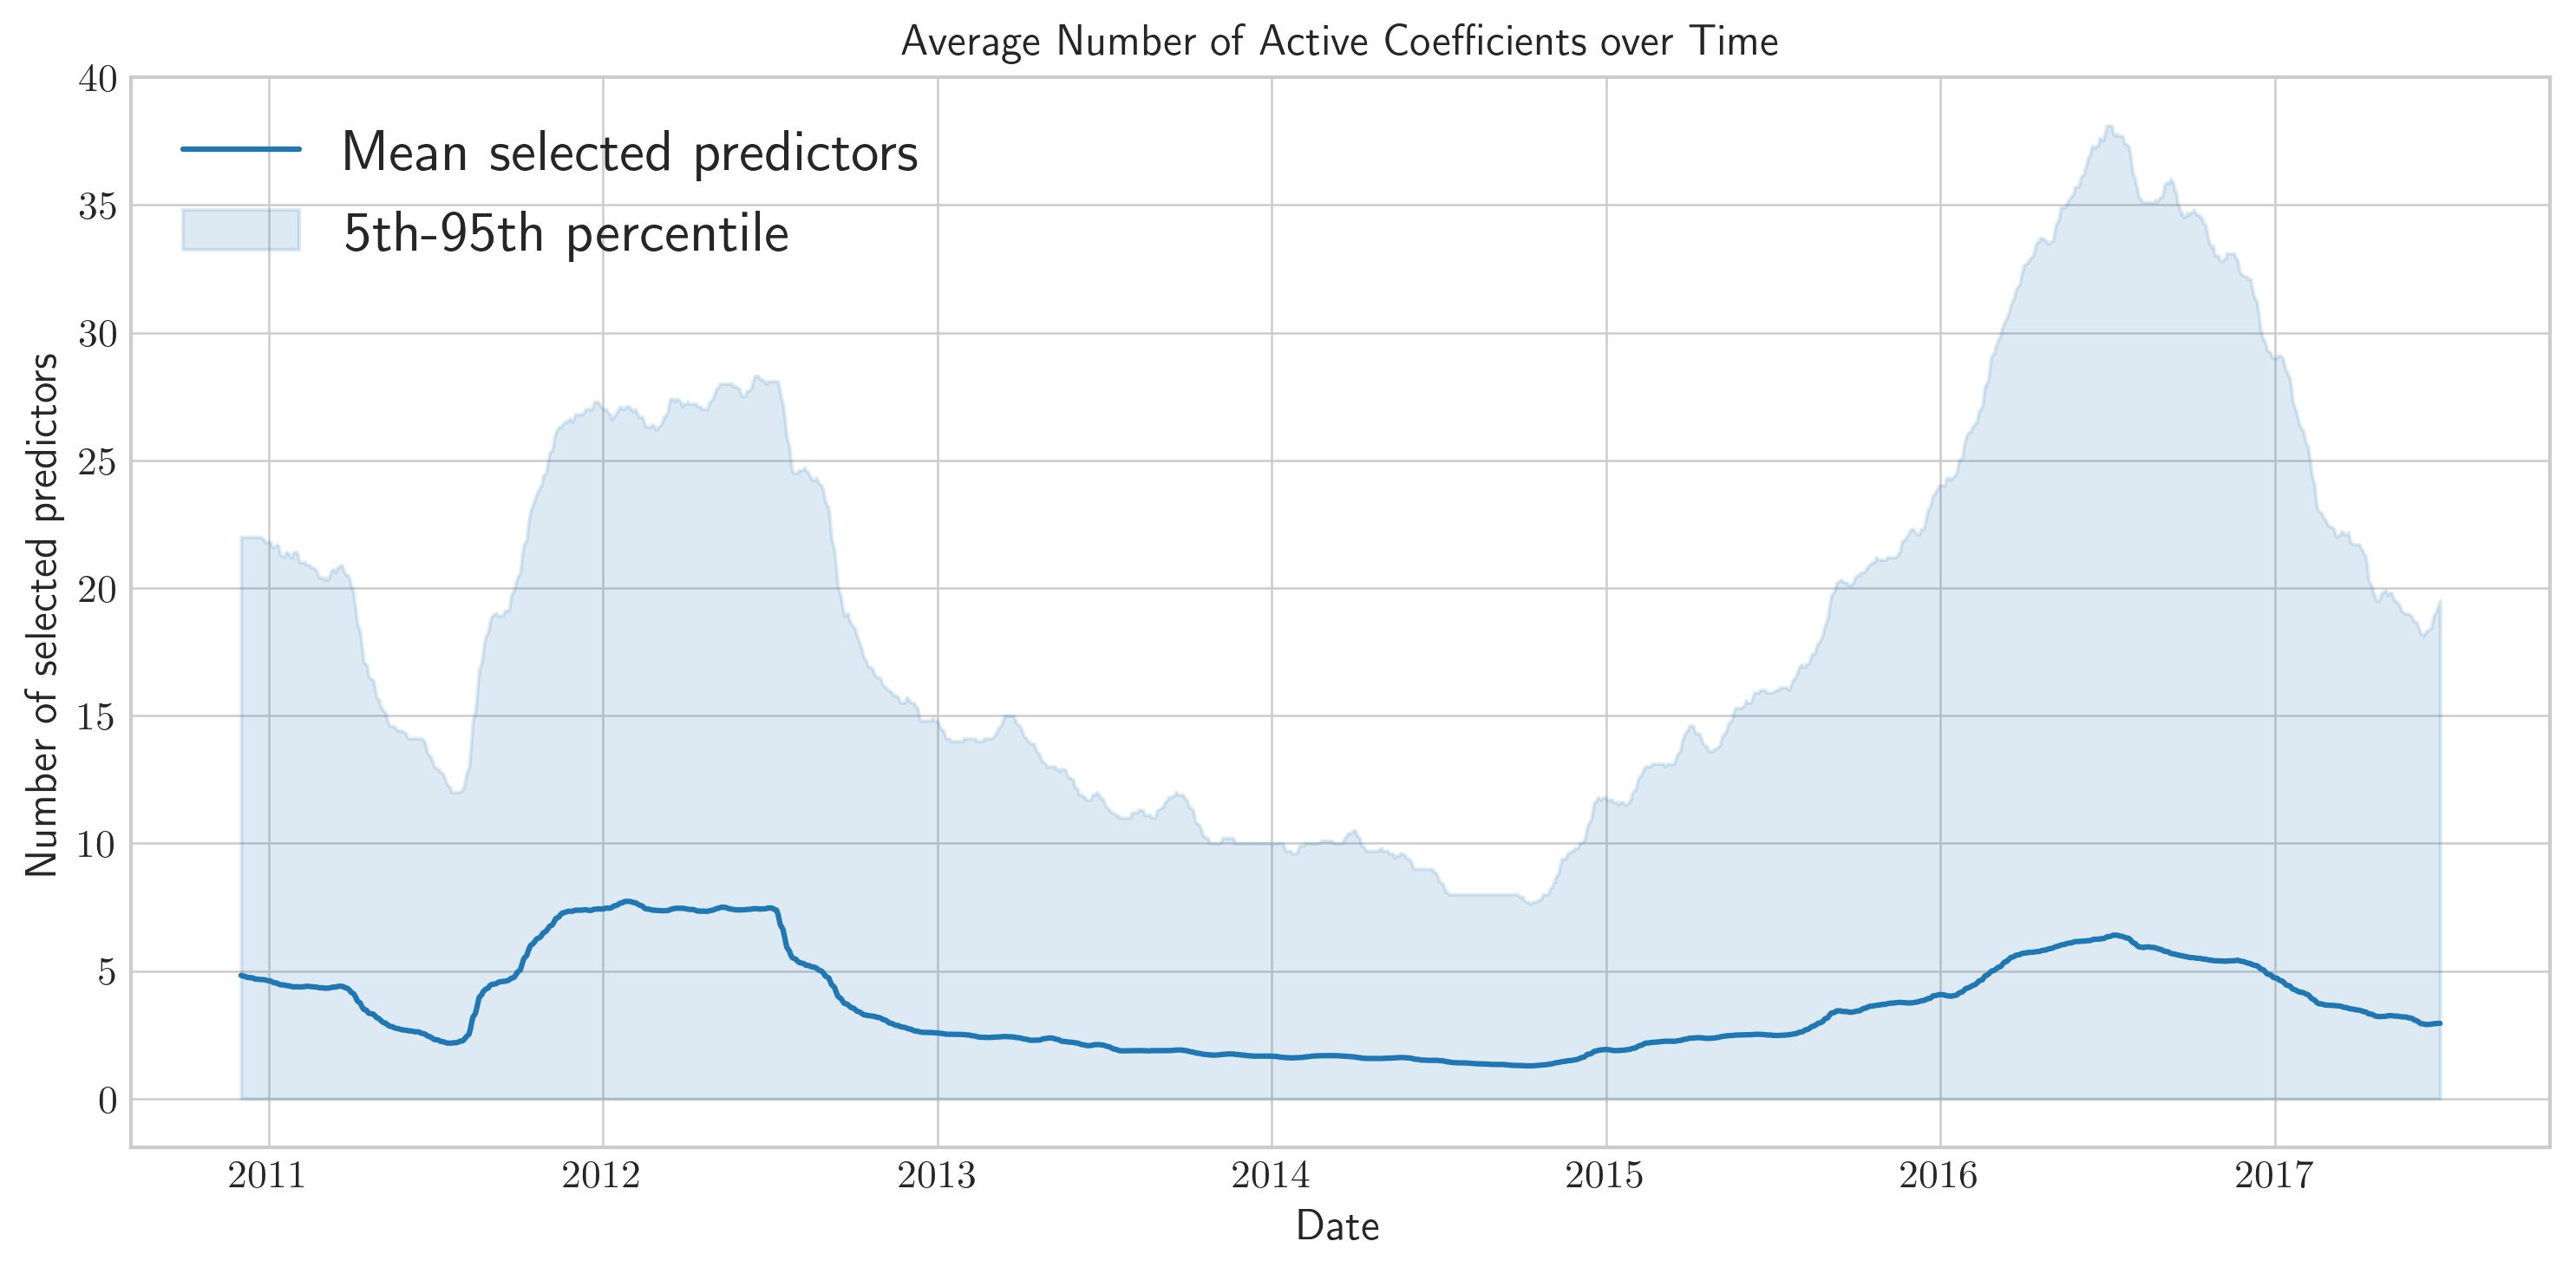
\includegraphics[width=0.7\textwidth]{active_coefficients_over_time.png}
    \caption{Time Variation in LASSO Selection Intensity}
    \label{fig:selection_rate_time}
    \begin{minipage}{\textwidth}
    \footnotesize
    % \textit{Note:} The figure plots the cross-sectional mean number of predictors selected by the LASSO on each trading day. The shaded region denotes the 10th--90th percentile range across stocks. All series are smoothed using a 21-day moving average. Vertical lines mark selected macro-financial events.
    \end{minipage}
\end{figure}

\paragraph{Cross-Sectional Variation.}

Proposition~\ref{prop:LASSO_estimate} implies that under a common penalty, stocks with more volatile returns should be more likely to generate non-zero LASSO coefficients. Figure~\ref{fig:avg_select} plots, for each stock, the mean LASSO selection rate against its idiosyncratic volatility $\hat{\sigma}_i$, measured as the standard deviation of Stage-2 residuals.
Stocks with a statistically significant $\hat{\kappa}$ estimate (at the 5\% level) are highlighted in red.
The relationship is strongly positive and convex: stocks with low idiosyncratic volatility are almost never selected, while the most volatile stocks are selected in upwards of 15\% of rolling windows.

\begin{figure}[h]
\centering
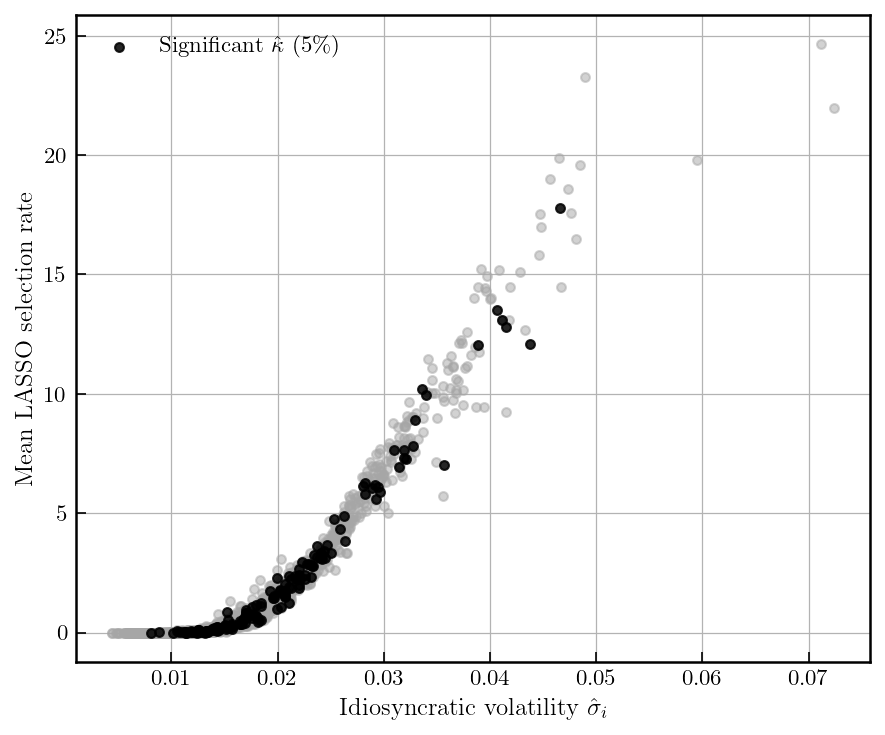
\includegraphics[width=0.7\textwidth]{scatter_idio_vol_selection_r2.png}
\caption{Mean LASSO Selection Rate vs.\ Idiosyncratic Volatility}
\label{fig:avg_select}
\end{figure}

% These patterns suggest that the estimated beliefs are sparse, episodic, and heterogeneous across stocks. The learning rule delivers some in-sample fit, while its out-of-sample performance remains weak, as documented above. This combination is consistent with the model's benchmark in which agents perceive temporary predictability from finite samples even though stable out-of-sample predictability is absent. The results also parallel the evidence in \citet{Chinco2019}, where return predictability appears in short-lived and shifting pockets rather than as a stable forecasting relation.

We next examine \emph{which} features the LASSO selects. 
Again, Proposition~\ref{prop:LASSO_estimate} provides a testable prediction: features with higher volatility should be selected less frequently.
However, since topic-attention innovations are standardized before entering the rolling estimation window, no feature is mechanically more likely to be selected than any other.
Selection should therefore be approximately uniform across features.
To test this, we define the mean selection rate as the fraction of stock-window observations for which the corresponding LASSO coefficient is non-zero.
We compute the rate for each of the 190 predictors. 

Figure~\ref{fig:topic_selection_freq} ranks the 190 candidate features by mean selection rate. Selection is moderately concentrated, with a Gini coefficient of 0.18, but remains dispersed. Every feature is selected at least once, and the most frequently selected feature, \textit{Announce plan}, is selected at $3.1$ times the equal-selection benchmark. The 10 macro-financial series are selected at a rate only marginally higher than the 180 news-topic features ($1.1\times$ on average), suggesting that the modest premium cannot be attributed to a structural advantage of macro series over news topics. The two most frequently selected features, \textit{Announce plan} and \textit{Financial reports}, are both news topics with clear economic interpretations as signals of corporate activity and earnings news.
Overall, no small subset of features dominates the learning rule. Instead, selection is dispersed, with moderate concentration in economically interpretable predictors. Appendix~\ref{app:robustness_sig_kappa} shows that the same pattern holds when the analysis is restricted to the stocks with a statistically significant $\hat{\kappa}$ estimate.

\begin{figure}[h]
    \centering
    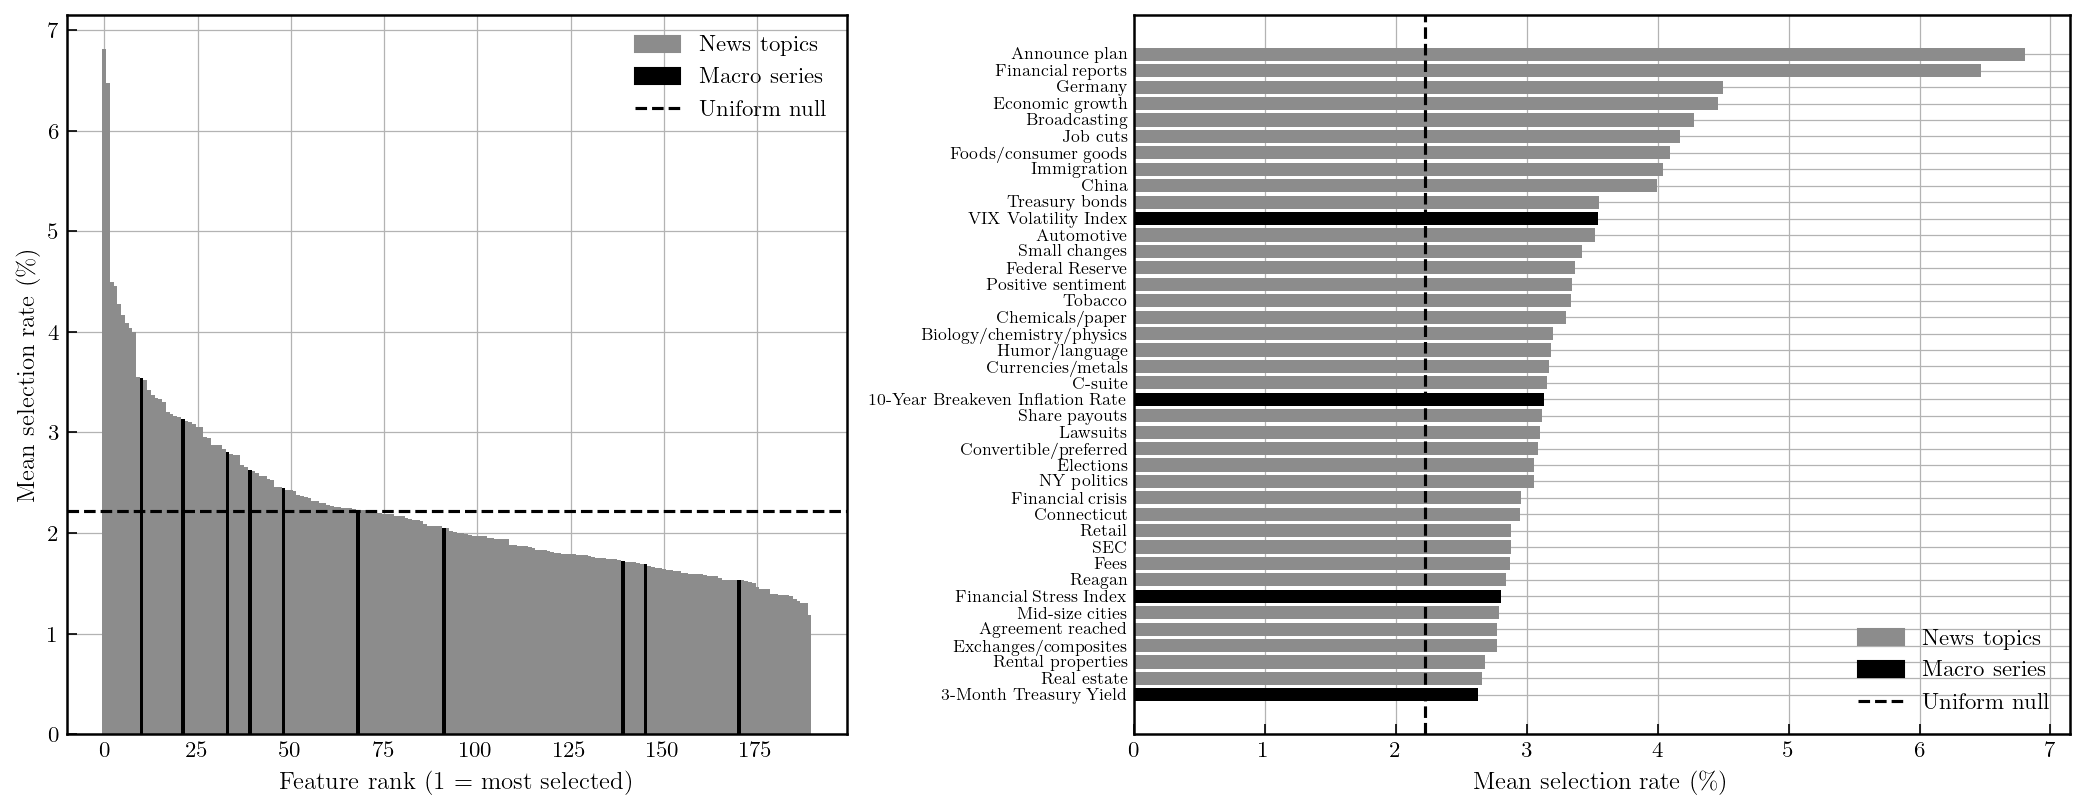
\includegraphics[width=\textwidth]{selection_frequency.png}
    \caption{LASSO Selection Frequency Across Features}
    \label{fig:topic_selection_freq}
    \begin{minipage}{\textwidth}
    \footnotesize
    \textit{Note:} Bars show mean feature selection rates, defined as the share of stock-days with a non-zero LASSO coefficient. Features are ordered by selection frequency; red bars denote macro-financial series and blue bars denote news topics. The dashed line marks the uniform-selection benchmark. The left panel shows all 190 features, while the right panel reports the top 30.
    \end{minipage}
\end{figure}

Figure~\ref{fig:topic_selection_by_stock} plots the distribution of average selected features per rolling window across the 1{,}296 estimation stocks. The distribution is strongly right-skewed, with a substantial mass near zero: approximately 40\% of stocks have an average selection rate below 0.3\%, consistent with the LASSO penalty being especially restrictive for lower-volatility stocks. Together with Figure~\ref{fig:topic_selection_freq}, these results show that sparsity is a structural feature of the data in two dimensions: agents typically select only a sparse subset of features for any individual stock, and the degree of selection varies substantially across the cross-section.


\begin{figure}[h]
    \centering
    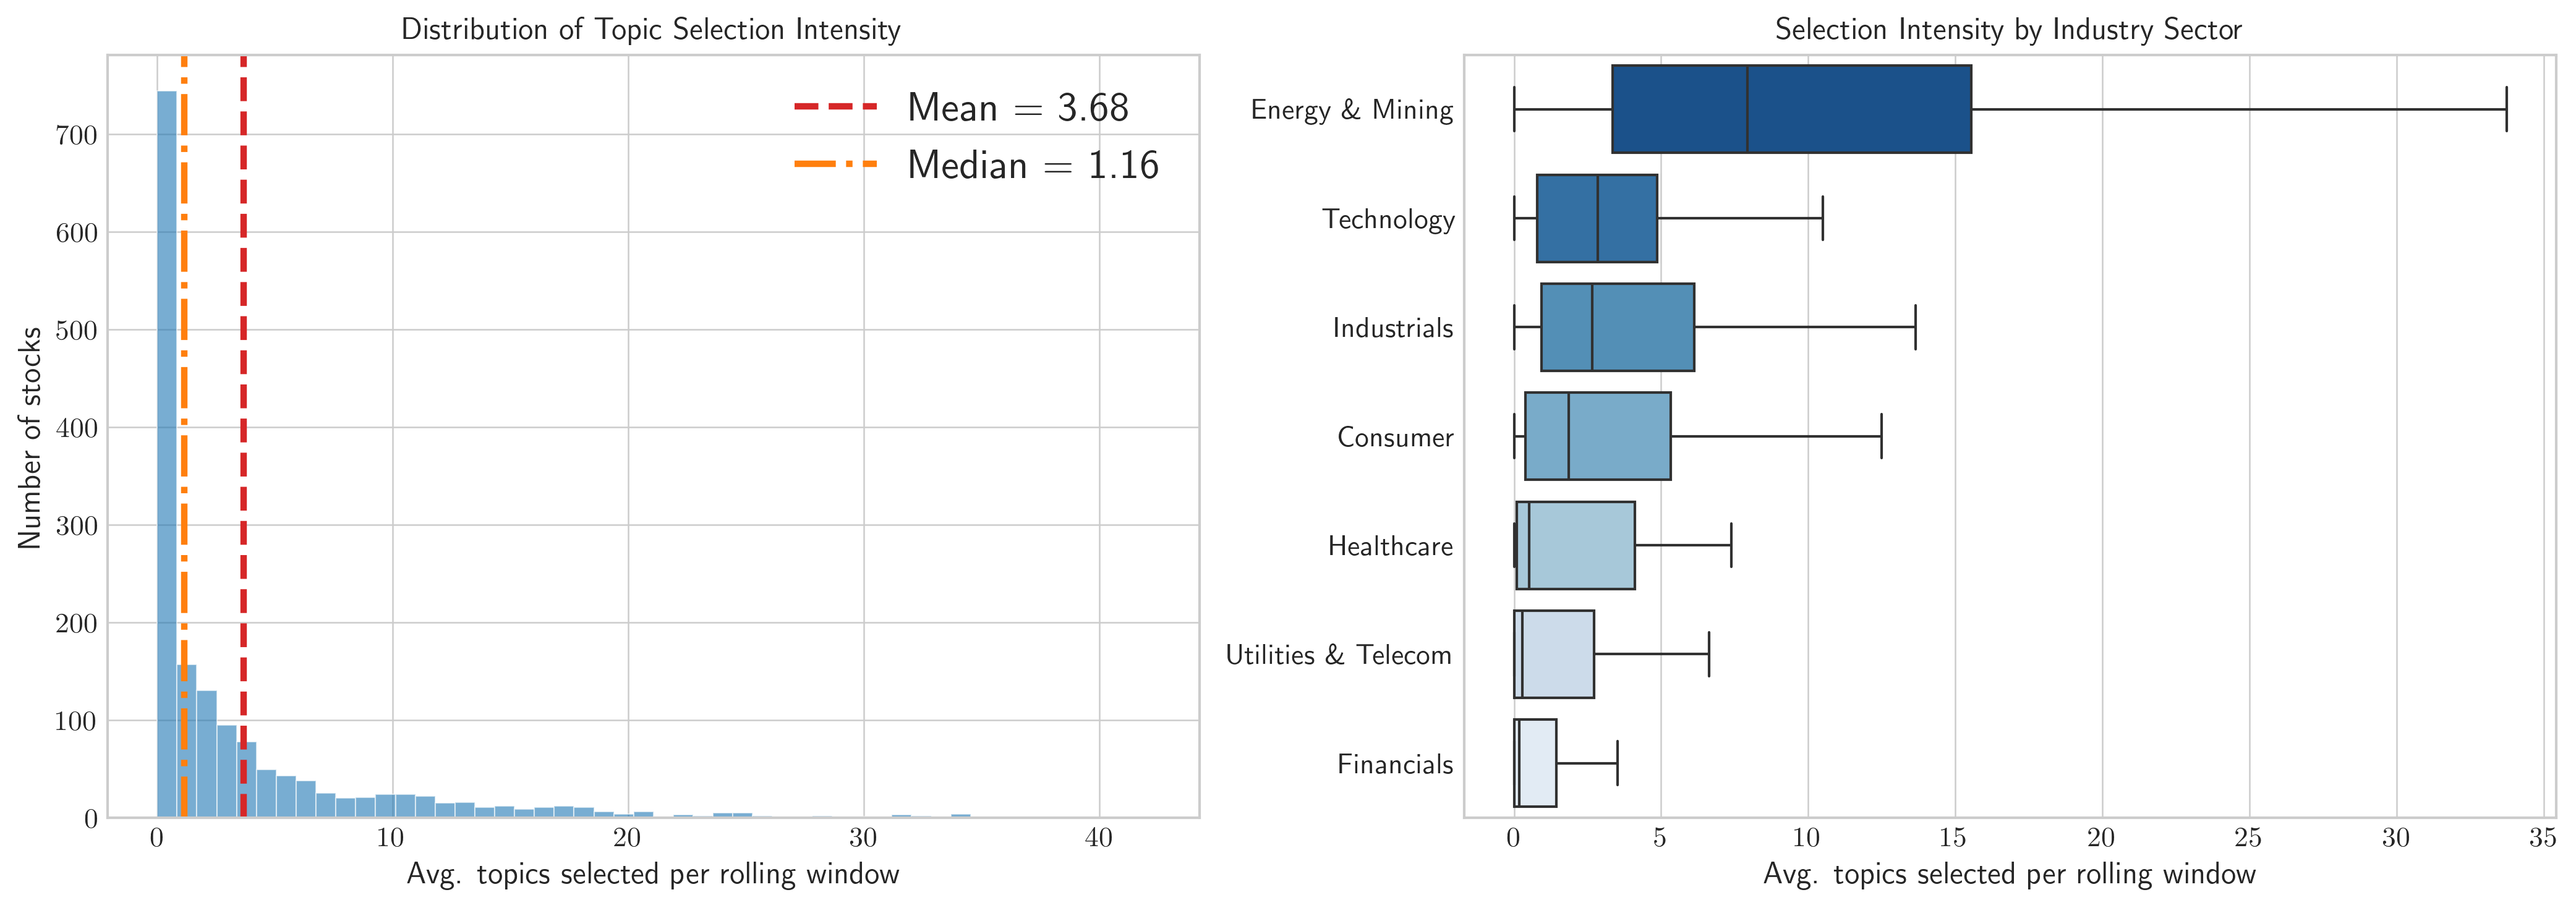
\includegraphics[width=\textwidth]{selection_intensity.png}
    \caption{LASSO Selection Intensity Across Stocks}
    \label{fig:topic_selection_by_stock}
    \begin{minipage}{\textwidth}
    \footnotesize
    \textit{Note:} Histogram of the average number of features selected per rolling window across the 1{,}296 estimation stocks. Dashed line: cross-sectional mean. Dotted line: median.
\end{minipage}
\end{figure}

\paragraph{Persistence.}

Figure~\ref{fig:topic_selection_persistence} shows that topic selection is highly persistent. Pooled across 547{,}907 selection episodes, the run-length distribution is strongly right-skewed: the median episode lasts only 4 windows, yet the 95th percentile reaches 79 windows and some episodes persist for over 600 windows. The survival curve declines from 73\% after one window to 18\% after 20 windows, before flattening into a heavy tail. 
To further quantify persistence, we define a selection indicator $s_{i,j,t} = \mathbf{1}(\hat{\beta}_{i,j,t} \neq 0)$ for each stock--feature pair $(i,j)$ and window $t$. The first-order autocorrelation of $s_{i,j,t}$, averaged across 72{,}882 active stock--feature pairs, is 0.89, decaying slowly to 0.73 at lag 5 and 0.46 at lag 20. While most episodes are short-lived, a minority of topic--stock pairs exhibits highly persistent selection, consistent with the self-reinforcing nature of the CMCE mechanism: a selected belief generates returns that sustain the selection signal until the rolling window rolls past the episode. This is in line with Remark~\ref{rem:persistence} in Section~\ref{sec:lasso}
Appendix~\ref{app:robustness_sig_kappa} confirms that the same pattern holds when restricting to stocks with a statistically significant $\hat{\kappa}$ estimate.

\begin{figure}[h]
    \centering
    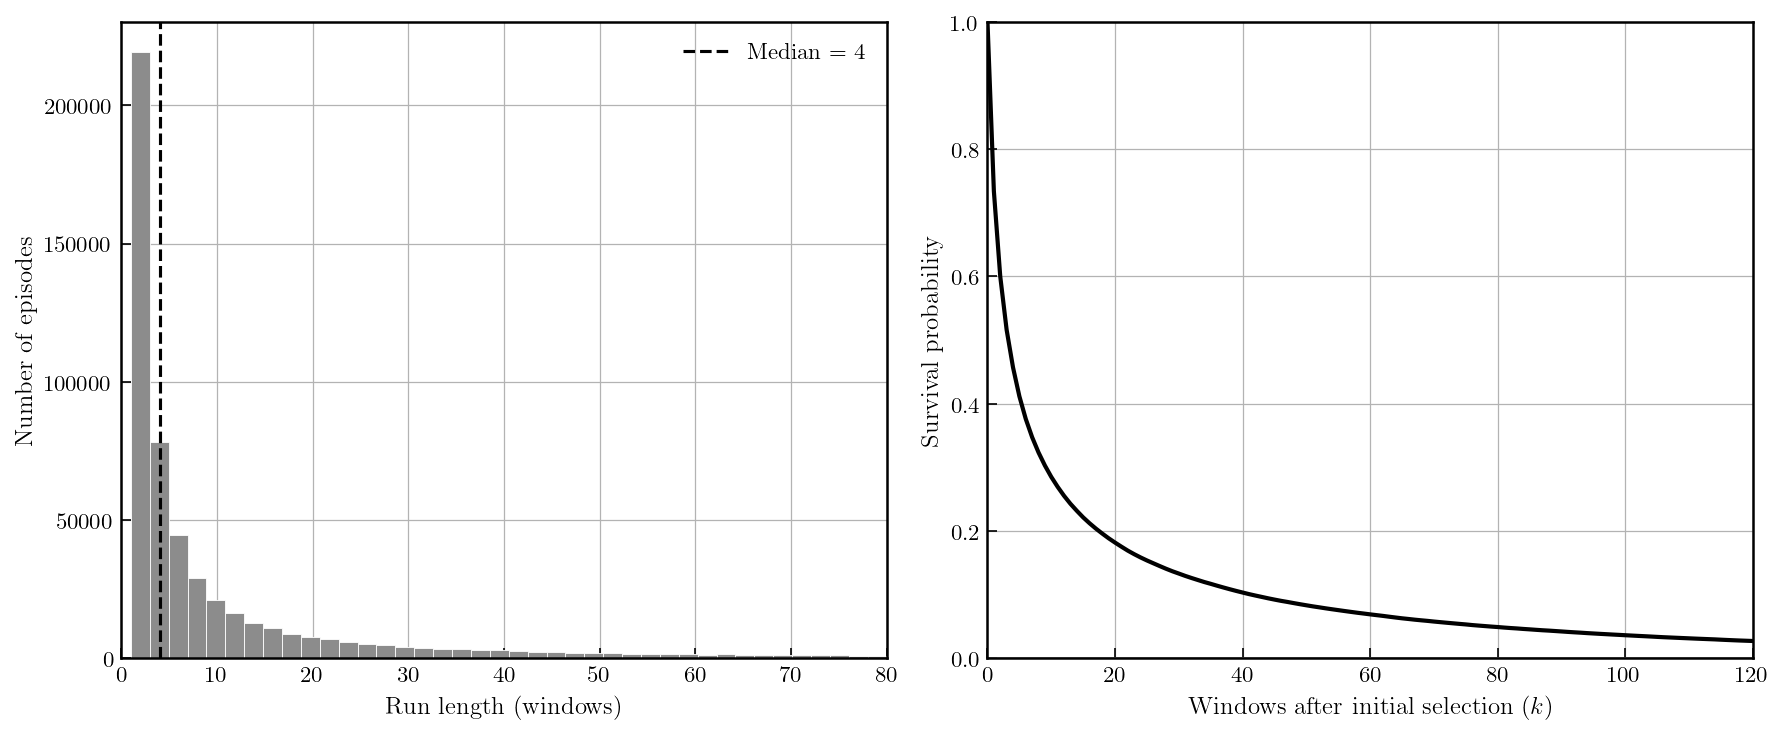
\includegraphics[width=\textwidth]{distribution_survival_autocorrelation.png}
    \caption{Persistence of Topic Selection Episodes}
    \label{fig:topic_selection_persistence}
    \begin{minipage}{\textwidth}
    \footnotesize
    \textit{Note:} \textbf{Left panel}: distribution of run lengths (consecutive windows a feature remains selected), pooled across 547{,}907 episodes and truncated at 80 windows. Dashed line marks the median ($=4$). \textbf{Right panel}: survival curve $P(\text{selected at }t+k \mid \text{selected at }t)$, estimated for each onset event and averaged across all stock--feature pairs. Sample: 1{,}296 stocks, 190 predictors, 1{,}626 trading days.
    \end{minipage}
\end{figure}

\subsection{Volatility, Uncertainty, and Selection}
\label{subsec:empirical_uncertainty_volatility}

\paragraph{Selection and Volatility.}

The model implies that LASSO selection should become more likely when the return process is more volatile. Under a fixed penalty parameter $\lambda$, higher return volatility increases the magnitude of sample return--predictor covariances and therefore raises the probability that estimated coefficients clear the selection threshold. By contrast, higher predictor volatility reduces standardized coefficient magnitudes and should lower selection probabilities. The empirical implication is therefore not simply that ``uncertainty'' raises selection in general, but more specifically that return-side uncertainty increases the likelihood of finite-sample relationships crossing the LASSO threshold.

Figure~\ref{fig:selection_rate_time} provides initial descriptive evidence. Feature selection becomes more frequent during periods of heightened aggregate uncertainty. The average number of selected predictors per stock-day is positively correlated with the VIX, a widely used measure of market uncertainty. The Pearson correlation between the two series is $r=0.358$ ($p<0.001$), indicating that periods of elevated market uncertainty are associated with higher rates of feature selection.

\paragraph{Time-series variation in aggregate selection intensity.}

We next examine what drives time-series variation in aggregate selection intensity. In the baseline CMCE equilibrium with constant idiosyncratic volatility $\sigma_u$, the expected selection rate is time invariant. Systematic co-movement between selection rates and observable volatility measures therefore points to variation outside the baseline model.

To decompose the sources of this variation, we first regress the aggregate selection rate $\bar{s}_t$ on two volatility proxies: the cross-sectional standard deviation of daily returns, $\sigma_{r,t}$, and average absolute topic activity, $\sigma_{x,t}$. The LASSO mechanism implies opposite signs for the two variables. Higher return volatility increases the magnitude of sample return--predictor covariances and raises the probability that coefficients clear the selection threshold. Higher predictor volatility, by contrast, lowers standardized coefficient magnitudes and should reduce selection. Consistent with these predictions, a regression with Newey--West standard errors using 20 lags yields $R^2=0.12$. The coefficient on return volatility is positive and significant, $\hat\beta_{\sigma_r}=0.188$ ($p<0.01$), while the coefficient on topic volatility is negative and significant, $\hat\beta_{\sigma_x}=-0.170$ ($p<0.01$).

To evaluate whether the observed time-series variation can be generated by the finite-sample properties of the model alone, we conduct an oracle simulation. We replace actual returns with i.i.d.\ draws from $\mathcal{N}(0,\hat\sigma_{u,i}^2)$ for 150 stocks and re-estimate the rolling LASSO using each stock's estimated penalty parameter and the same window length, $s=231$. Under constant-variance i.i.d.\ noise, the model predicts a time invariant aggregate selection rate. This is what we find: the standard deviation of the simulated selection rate is 19 times smaller than in the data, and the Spearman correlation between actual and simulated selection rates is close to zero, $\rho=0.02$ ($p=0.31$). Thus, i.i.d.\ noise calibrated to the empirical residual variance cannot account for the observed time-series variation in selection intensity.

% \begin{figure}[H]
%     \centering
%     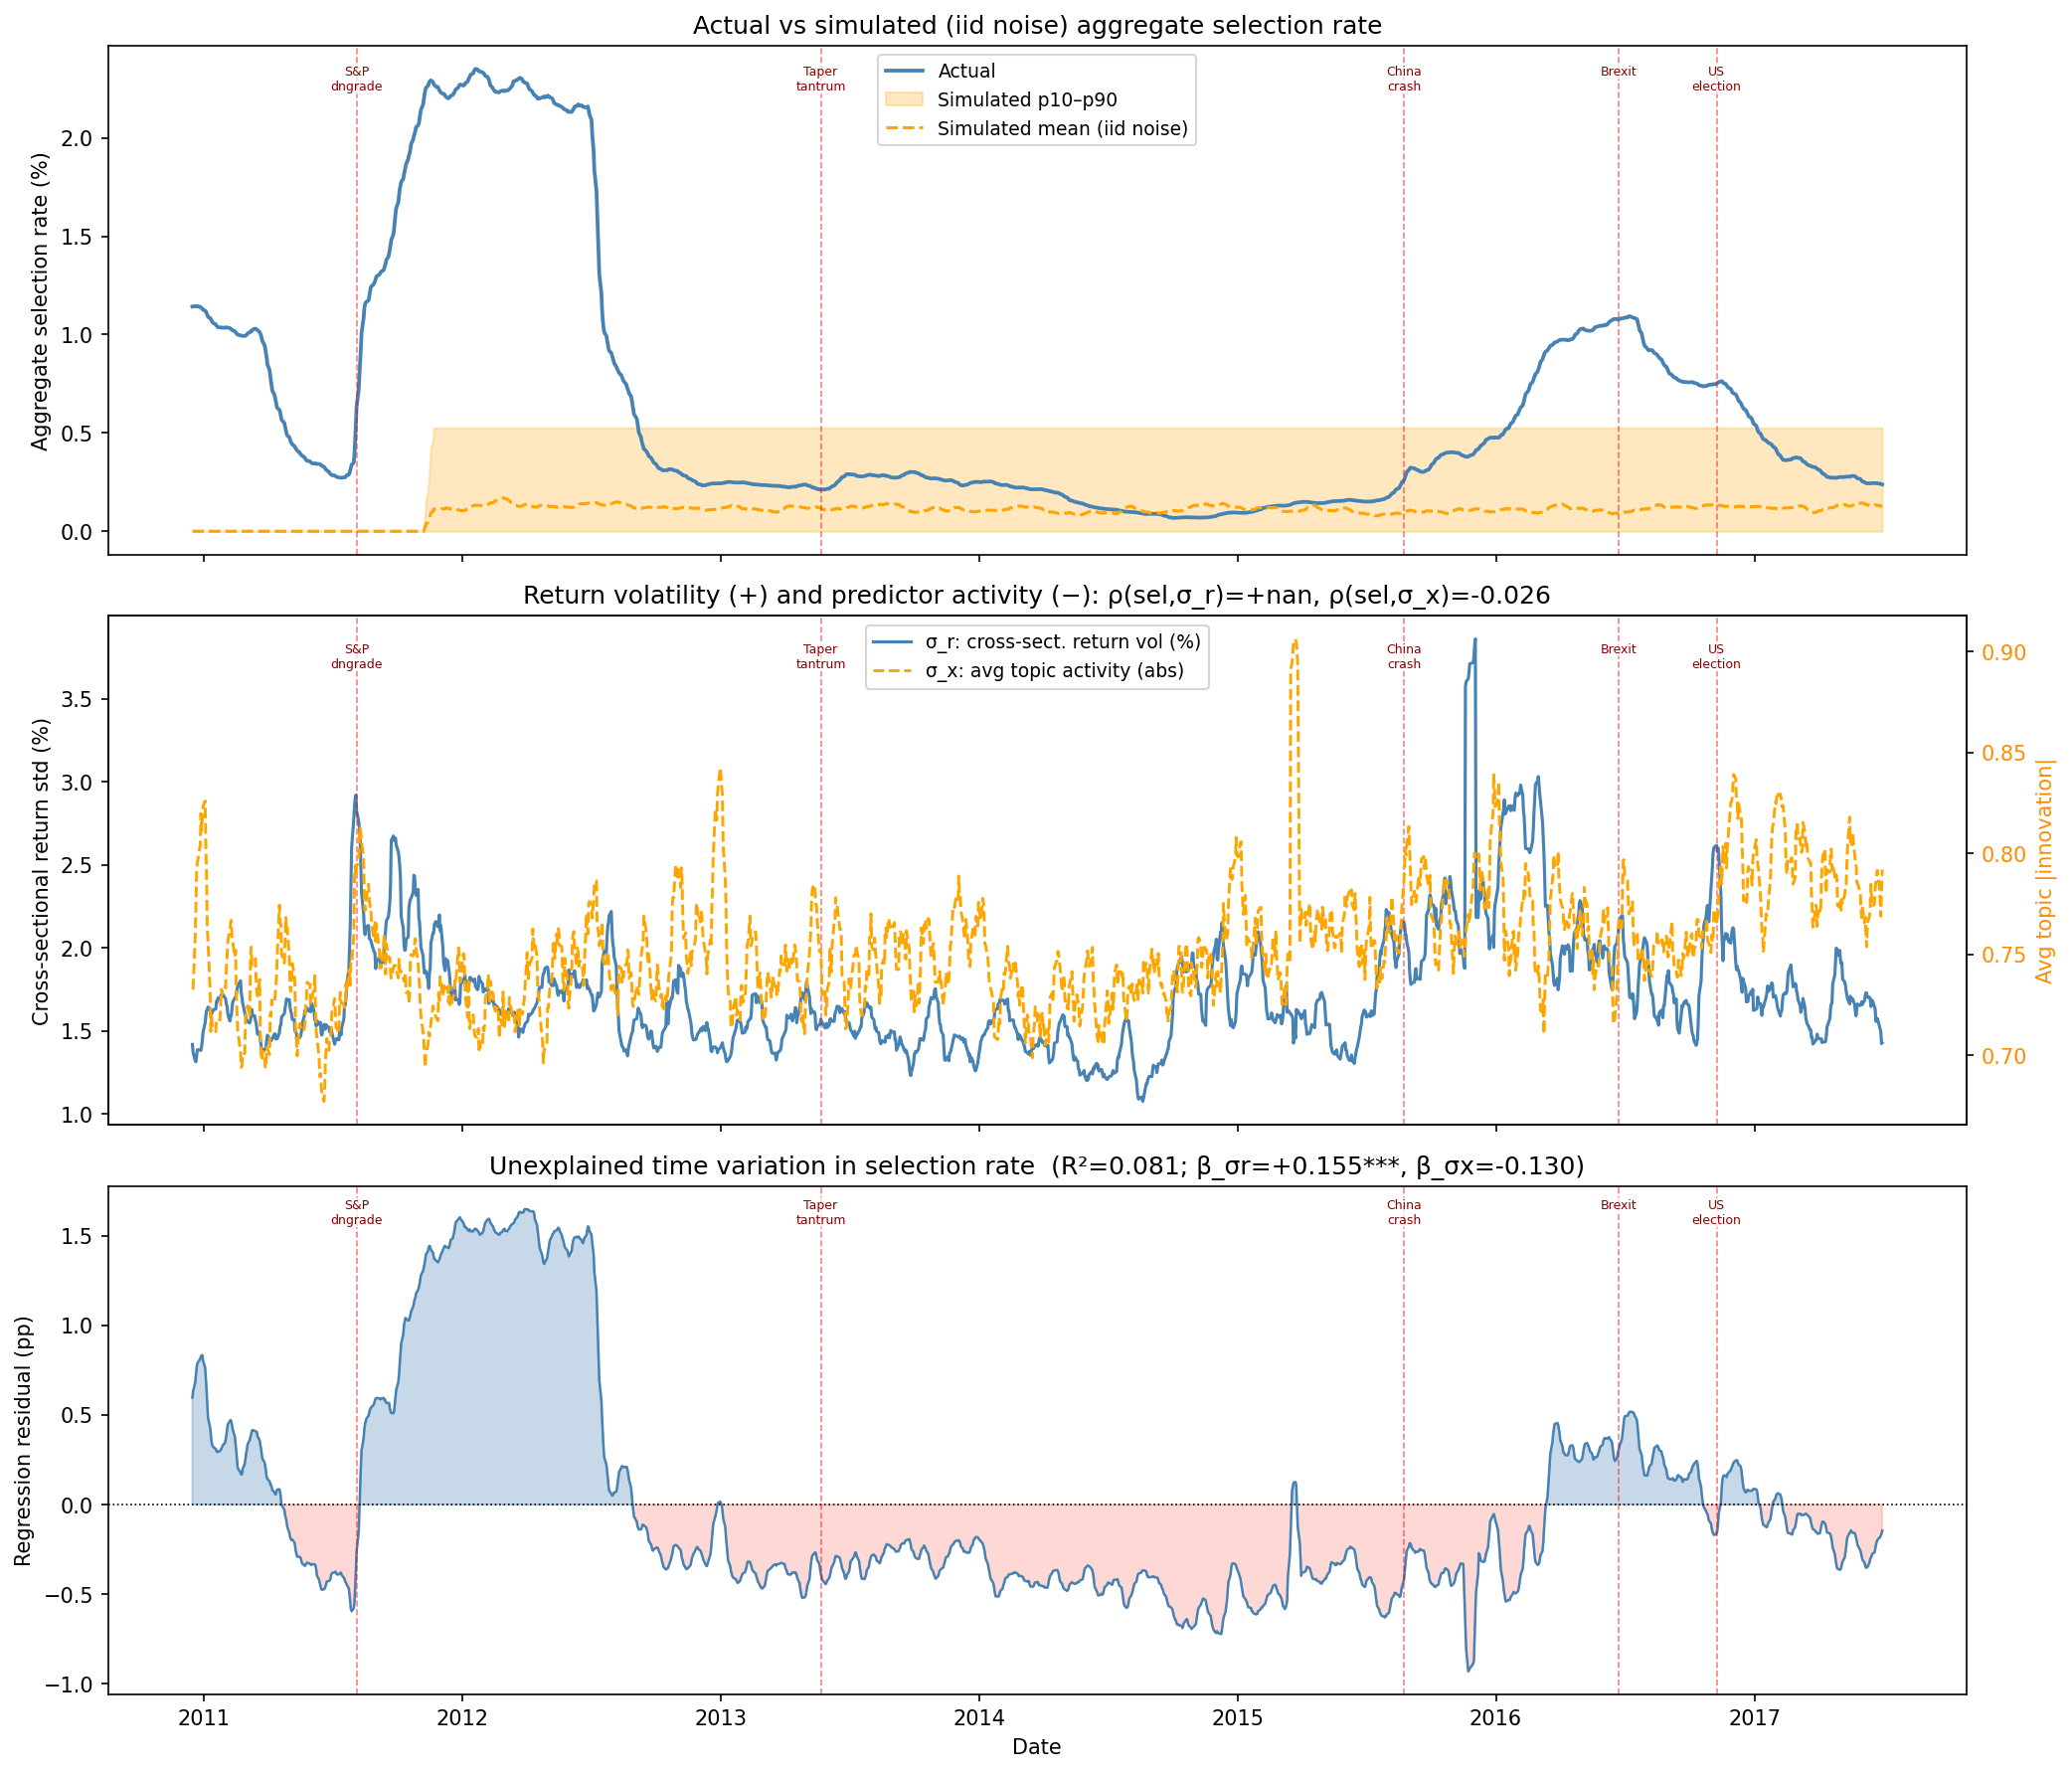
\includegraphics[width=\textwidth]{selection_rate_decomposition.png}
%     \caption{Time-Series Variation in Aggregate Selection Rates}
%     \label{fig:selection_rate_decomposition}
%     \begin{minipage}{\textwidth}
%     \footnotesize
%     \textit{Note:} The top panel compares the actual aggregate selection rate with the i.i.d.\ oracle simulation. The middle panel plots cross-sectional return volatility, $\sigma_{r,t}$, and average absolute topic activity, $\sigma_{x,t}$. The bottom panel reports residuals from the regression
%     $\bar{s}_t = a + b_1\sigma_{r,t} + b_2\sigma_{x,t} + \varepsilon_t$,
%     estimated with Newey--West standard errors using 20 lags. Red dashed lines mark selected macroeconomic events.
%     \end{minipage}
% \end{figure}

\paragraph{Conditional volatility and selection spikes.}

The large gap between actual and simulated selection-rate volatility suggests that the baseline model misses an important feature of the data. We therefore allow the residual return component to exhibit conditional heteroskedasticity. Economically, the residual $u_{i,t}$ captures return variation not spanned by the topic predictors, including earnings surprises, idiosyncratic demand shocks, and liquidity effects. Such residual variation is likely to be state dependent: during periods of macroeconomic stress, both the magnitude and the common component of firm-level shocks tend to increase.
We model this channel using
\[
u_{i,t} = \sigma_{m,t}\eta_t^{(m)} + \tilde\sigma_i\eta_{i,t}^{(i)},
\]
where $\sigma_{m,t}$ follows a GARCH$(1,1)$ process fitted to value-weighted market returns. When conditional market volatility rises, many firms simultaneously experience larger residual shocks. This increases the probability that rolling-window coefficients cross the LASSO threshold, generating aggregate selection spikes even in the absence of stable return predictability.

We quantify this mechanism by simulating 150 stocks with GARCH residuals calibrated to each stock's market beta and idiosyncratic volatility, and then re-running the same rolling LASSO. Relative to the i.i.d.\ oracle, the GARCH oracle matches the data substantially better. The ratio of actual to simulated selection-rate volatility falls from 19.0 under i.i.d.\ noise to 1.32 under GARCH noise. The Spearman correlation between actual and simulated aggregate selection rates rises from $\rho=0.02$ ($p=0.31$) to $\rho=0.38$ ($p<0.0001$). Replacing raw return volatility with the GARCH conditional volatility, $\sigma_{m,t}$, in the regression increases the explanatory power from $R^2=0.12$ to $R^2=0.18$, with $\hat\beta_{\sigma_m}=0.242$ ($p<0.01$) and $\hat\beta_{\sigma_x}=-0.132$ ($p<0.01$).

% \begin{figure}[H]
%     \centering
%     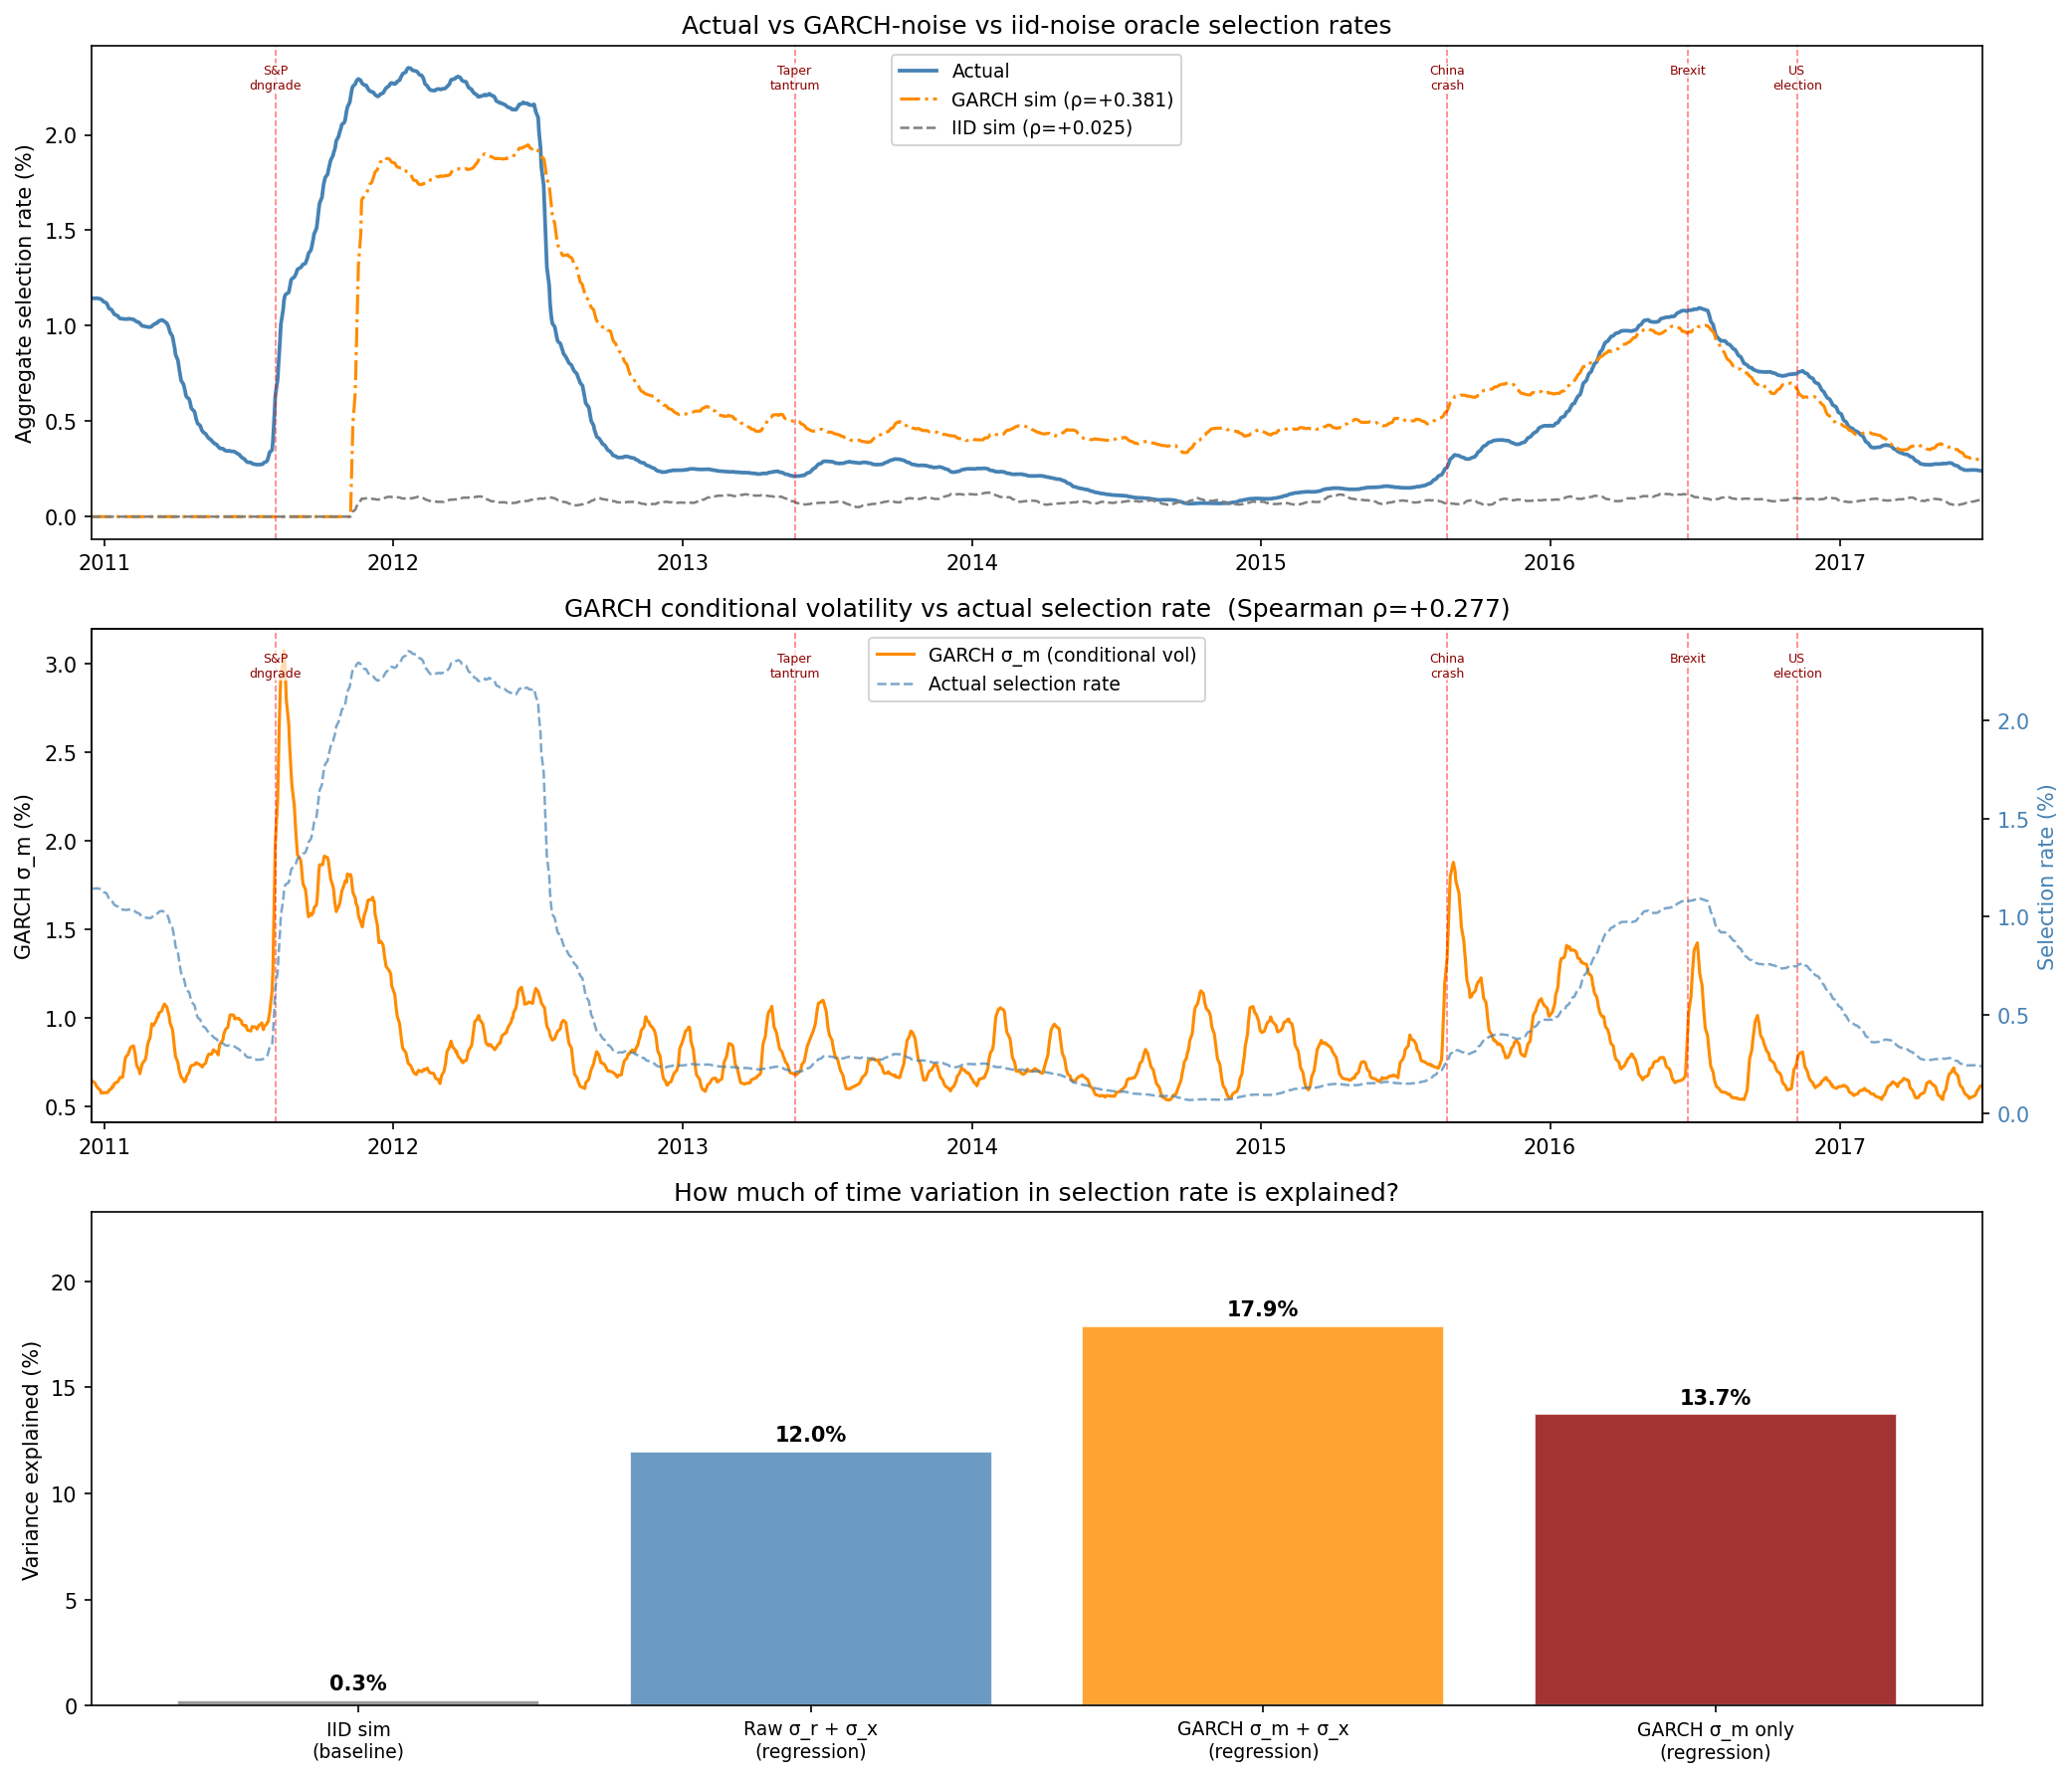
\includegraphics[width=\textwidth]{garch_selection_oracle.png}
%     \caption{Conditional Volatility and Aggregate Selection Rates}
%     \label{fig:garch_oracle}
%     \begin{minipage}{\textwidth}
%     \footnotesize
%     \textit{Note:} The top panel compares the actual aggregate selection rate with the GARCH oracle and the i.i.d.\ oracle. The middle panel plots the GARCH conditional volatility $\hat\sigma_{m,t}$ from a GARCH$(1,1)$ model fitted to daily value-weighted market returns, together with the actual selection rate. The bottom panel reports the fraction of selection-rate variation explained by the i.i.d.\ oracle, the raw-volatility regression, the GARCH-volatility regression, and the GARCH volatility alone. The estimated GARCH persistence parameter is $\hat\alpha+\hat\beta=0.96$.
%     \end{minipage}
% \end{figure}

Taken together, these results indicate that episodic selection spikes are closely linked to time-varying return uncertainty with a common component. The LASSO does not select more topics during high-volatility periods simply because topic activity increases. Rather, conditional return volatility raises the probability that sample relationships cross the selection threshold. The volatility results therefore explain when selection becomes more likely, but not which stock--topic pairs are selected.

\paragraph{Firm-level uncertainty and selection.}

We next ask whether the positive association between uncertainty and selection also appears at the firm level. To do so, we construct a firm-quarter uncertainty index from firms' 10-K filings, measured as the frequency of uncertainty-related terms per 10,000 words, and match it to the quarterly average LASSO selection rate of each firm. Since the distribution of textual uncertainty is highly skewed, all specifications use the log-transformed uncertainty index, standardized within each quarter.

Table~\ref{tab:uncertainty_selection} reports the results. Column~(1) includes firm fixed effects, absorbing all time-invariant firm characteristics, while Column~(2) additionally controls for quarter fixed effects, removing aggregate time-series variation common to all firms. In both specifications a one-standard-deviation increase in log textual uncertainty is associated with a positive and statistically significant increase in the quarterly LASSO selection rate. The coefficient in Column~(1) is 0.18 percentage points ($t=2.07$), indicating that firms with higher reported uncertainty tend to exhibit more active feature selection. Adding quarter fixed effects in Column~(2) yields a coefficient of 0.15 percentage points ($t=1.79$), confirming that the relation holds within firms over time after controlling for aggregate quarterly conditions.
\begin{table}[H]
\centering
\caption{Firm-Level Uncertainty and LASSO Selection}
\label{tab:uncertainty_selection}

\begin{tabular}{lcc}
\toprule
& \multicolumn{2}{c}{Dependent Variable: Selection Rate} \\
\cmidrule(lr){2-3}
& (1) & (2) \\
\midrule
Log Uncertainty Index
    & 0.0018** & 0.0015* \\
    & (0.0009) & (0.0008) \\
\midrule
Firm FE
    & Yes & Yes \\
Quarter FE
    & No  & Yes \\
\midrule
Observations
    & 20,467 & 20,467 \\
Firms
    & 806 & 806 \\
Quarters
    & 26 & 26 \\
$R^2$
    & 0.001 & 0.001 \\
\bottomrule
\end{tabular}

\vspace{0.15cm}
\begin{minipage}{0.95\textwidth}
\footnotesize
\textit{Note:} The dependent variable is the quarterly average LASSO selection rate. The uncertainty index is constructed from 10-K filings, log-transformed, and standardized to have mean zero and unit standard deviation. Both specifications are estimated by panel OLS with firm fixed effects; Column~(2) additionally includes quarter fixed effects. Standard errors are clustered at the firm level. $^{*}p<0.10$, $^{**}p<0.05$, $^{***}p<0.01$.
\end{minipage}
\end{table}
Overall, the firm-level results provide complementary evidence that selection is more common in uncertain information environments. The central mechanism is the volatility channel documented above. Return-side uncertainty raises the probability that finite-sample relationships cross the LASSO threshold.



